\chapter{PENGUJIAN DAN EVALUASI}
	Pada bab ini akan dibahas uji coba dan evaluasi dari sistem yang telah dibuat. Sistem akan diuji coba fungsionalitas dan performanya dengan menjalankan skenario uji coba yang sudah ditentukan. Uji coba dilakukan untuk mengetahui hasil dari sistem ini sehingga dapat menjawab rumusan masalah pada tugas akhir ini.    
	
\section{Lingkungan Uji Coba}
	Lingkungan pengujian menggunakan komponen-komponen yang terdiri dari: satu \textit{server docker host}, satu \textit{server login}, dan tiga komputer penguji.Semua komputer penguji menggunakan enam buah desktop dengan sistem operasi Ubuntu 16.04
	. Pengujian dilakukan di Laboratoriom Arsitektur dan Jaringan Komputer Jurusan Teknik Informatika ITS. \\
    \indent Spesifikasi untuk setiap komponen yang digunakan ditunjukkan pada Tabel \ref{spesifikasidockerhost} untuk \textit{docker host}, Tabel \ref{spesifikasihalamanlogin} untuk \textit{server} halaman login, Tabel \ref{spesifikasikomputerpenguji1} untuk Komputer Penguji 1, Tabel \ref{spesifikasikomputerpenguji2} untuk Komputer Penguji 2, Tabel \ref{spesifikasikomputerpenguji3} untuk Komputer Penguji 3, Tabel \ref{spesifikasikomputerpenguji4} untuk Komputer Penguji 4, Tabel \ref{spesifikasikomputerpenguji5} untuk Komputer Penguji 5, dan Tabel \ref{spesifikasikomputerpenguji6} untuk Komputer Penguji 6.

\begin{enumerate}
	\item \textbf{\textit{Server} Untuk \textit{Docker Host}}
	\begin{longtable}{|l|l|}
		\caption{\textit{Server} Untuk \textit{Docker Host}}
		\label{spesifikasidockerhost} \\
		\hline
		\textbf{Perangkat Keras}      & \begin{tabular}[c]{@{}l@{}} Processor Intel(R) Core(TM) \\ i5-2120 CPU @ 3.30GHz\end{tabular} \\ \cline{2-2} 
		& RAM 8GB	\\ \cline{2-2} 
		& Hard disk 500GB \\ \hline
		\textbf{Perangkat Lunak}      & Linux Mint 18.03 64 bit \\ \cline{2-2} 
		& Docker-CE versi 1.13.1. \\ \cline{2-2} 
		& MySQL versi 5.7.18. \\ \cline{2-2} 
		& Iptables versi 1.6. \\ \cline{2-2} 
		& Python versi 3.5.2. \\ \cline{2-2} 
		& Flask versi 1.0.2.\\ \hline
		\textbf{Konfigurasi Jaringan} & IP address : 10.151.36.134 \\ \cline{2-2} 
		& Netmask : 255.255.255.0 \\ \cline{2-2} 
		& Gateway : 10.151.36.1 \\ \cline{2-2} 
		& Hostname : X450LD \\ \hline
	\end{longtable}
	
	\item \textbf{\textit{Server} Untuk Halaman Login}
	\begin{longtable}{|l|l|}
		\caption{\textit{Server} Untuk Halaman Login}
		\label{spesifikasihalamanlogin} \\
		\hline
		\textbf{Perangkat Keras}      & \begin{tabular}[c]{@{}l@{}} Processor Intel(R) Core(TM)2Duo \\ CPU E7200 @ 2.53GHz\end{tabular} \\ \cline{2-2} 
		& RAM 1GB	\\ \cline{2-2} 
		& Hard disk 20GB \\ \hline
		\textbf{Perangkat Lunak}      & Ubuntu 16.04 64 bit \\ \cline{2-2} 
		& Nginx versi 1.10.3. \\ \cline{2-2} 
		& Gunicorn versi 19.9.1. \\ \cline{2-2} 
		& Supervisor versi 3.2. \\ \cline{2-2} 
		& Python versi 3.5.2. \\ \cline{2-2} 
		& Flask versi 1.0.2.\\ \hline
		\textbf{Konfigurasi Jaringan} & IP address : 10.151.36.173 \\ \cline{2-2} 
		& Netmask : 255.255.255.0 \\ \cline{2-2} 
		& Gateway : 10.151.36.1 \\ \cline{2-2} 
		& Hostname : SERVERLOGIN \\ \hline
	\end{longtable}
	
	\item \textbf{Komputer Penguji}
	\begin{enumerate}
		\item \textbf{Komputer Penguji 1}
		\begin{longtable}{|l|l|}
			\caption{Komputer Penguji 1}
			\label{spesifikasikomputerpenguji1} \\
			\hline
			\textbf{Perangkat Keras}      & \begin{tabular}[c]{@{}l@{}} Processor Intel(R) Core(TM) \\ i5-2120 CPU @ 3.30GHz\end{tabular} \\ \cline{2-2} 
			& RAM 8GB	\\ \cline{2-2} 
			& Hard disk 500GB \\ \hline
			\textbf{Perangkat Lunak}      & Ubuntu 16.04 64 bit \\ \cline{2-2} 
			& Firefox Quantum versi 60.0.1.\\ \hline
			\textbf{Konfigurasi Jaringan} & IP address : 10.151.36.33 \\ \cline{2-2} 
			& Netmask : 255.255.255.0 \\ \cline{2-2} 
			& Gateway : 10.151.36.134 \\ \cline{2-2} 
			& Hostname : DRONA \\ \hline
		\end{longtable}
		
		\item \textbf{Komputer Penguji 2}
		\begin{longtable}{|l|l|}
			\caption{Komputer Penguji 2}
			\label{spesifikasikomputerpenguji2} \\
			\hline
			\textbf{Perangkat Keras}      & \begin{tabular}[c]{@{}l@{}} Processor Intel(R) Core(TM) \\ i3-2120 CPU @ 3.30GHz\end{tabular} \\ \cline{2-2} 
			& RAM 6GB	\\ \cline{2-2} 
			& Hard disk 1TB \\ \hline
			\textbf{Perangkat Lunak}      & Ubuntu 16.04 64 bit \\ \cline{2-2} 
			& Firefox Quantum versi 60.0.1.\\ \hline
			\textbf{Konfigurasi Jaringan} & IP address : 10.151.36.34 \\ \cline{2-2} 
			& Netmask : 255.255.255.0 \\ \cline{2-2} 
			& Gateway : 10.151.36.134 \\ \cline{2-2} 
			& Hostname : BHISMA \\ \hline
		\end{longtable}
		\pagebreak
		
		\item \textbf{Komputer Penguji 3}
		\begin{longtable}{|l|l|}
			\caption{Komputer Penguji 3}
			\label{spesifikasikomputerpenguji3} \\
			\hline
			\textbf{Perangkat Keras}      & \begin{tabular}[c]{@{}l@{}} Processor Intel(R) Core(TM) \\ i3-2120 CPU @ 3.30GHz\end{tabular} \\ \cline{2-2} 
			& RAM 4GB	\\ \cline{2-2} 
			& Hard disk 250GB \\ \hline
			\textbf{Perangkat Lunak}      & Ubuntu 16.04 64 bit \\ \cline{2-2} 
			& Firefox Quantum versi 60.0.1.\\ \hline
			\textbf{Konfigurasi Jaringan} & IP address : 10.151.36.33 \\ \cline{2-2} 
			& Netmask : 255.255.255.0 \\ \cline{2-2} 
			& Gateway : 10.151.36.134 \\ \cline{2-2} 
			& Hostname : ARJUNA \\ \hline
		\end{longtable}
		
		\item \textbf{Komputer Penguji 4}
		\begin{longtable}{|l|l|}
			\caption{Komputer Penguji 4}
			\label{spesifikasikomputerpenguji4} \\
			\hline
			\textbf{Perangkat Keras}      & \begin{tabular}[c]{@{}l@{}} Processor Intel(R) Core(TM) \\ i3-2120 CPU @ 3.30GHz\end{tabular} \\ \cline{2-2} 
			& RAM 8GB	\\ \cline{2-2} 
			& Hard disk 1TB \\ \hline
			\textbf{Perangkat Lunak}      & Ubuntu 16.04 64 bit \\ \cline{2-2} 
			& Firefox Quantum versi 60.0.1.\\ \hline
			\textbf{Konfigurasi Jaringan} & IP address : 10.151.36.38 \\ \cline{2-2} 
			& Netmask : 255.255.255.0 \\ \cline{2-2} 
			& Gateway : 10.151.36.134 \\ \cline{2-2} 
			& Hostname : KRESNA \\ \hline
		\end{longtable}
		\pagebreak
		
		\item \textbf{Komputer Penguji 5}
		\begin{longtable}{|l|l|}
			\caption{Komputer Penguji 5}
			\label{spesifikasikomputerpenguji5} \\
			\hline
			\textbf{Perangkat Keras}      & \begin{tabular}[c]{@{}l@{}} Processor Intel(R) Core(TM)2Duo \\ CPU E7200 @ 2.53GHz\end{tabular} \\ \cline{2-2} 
			& RAM 2GB	\\ \cline{2-2} 
			& Hard disk 120GB \\ \hline
			\textbf{Perangkat Lunak}      & Ubuntu 16.04 64 bit \\ \cline{2-2} 
			& Firefox Quantum versi 60.0.1.\\ \hline
			\textbf{Konfigurasi Jaringan} & IP address : 10.151.36.39 \\ \cline{2-2} 
			& Netmask : 255.255.255.0 \\ \cline{2-2} 
			& Gateway : 10.151.36.134 \\ \cline{2-2} 
			& Hostname : NARASOMA \\ \hline
		\end{longtable}
		
		\item \textbf{Komputer Penguji 6}
		\begin{longtable}{|l|l|}
			\caption{Komputer Penguji 6}
			\label{spesifikasikomputerpenguji6} \\
			\hline
			\textbf{Perangkat Keras}      & \begin{tabular}[c]{@{}l@{}} Processor Intel(R) Core(TM)2Duo \\ CPU E7200 @ 2.53GHz\end{tabular} \\ \cline{2-2} 
			& RAM 2GB	\\ \cline{2-2} 
			& Hard disk 120GB \\ \hline
			\textbf{Perangkat Lunak}      & Ubuntu 16.04 64 bit \\ \cline{2-2} 
			& Firefox Quantum versi 60.0.1.\\ \hline
			\textbf{Konfigurasi Jaringan} & IP address : 10.151.36.41 \\ \cline{2-2} 
			& Netmask : 255.255.255.0 \\ \cline{2-2} 
			& Gateway : 10.151.36.134 \\ \cline{2-2} 
			& Hostname : ANGGADA \\ \hline
		\end{longtable}
		
	\end{enumerate}
\end{enumerate}
			
			Untuk gambar arsitektur dari setiap komponen yang digunakan dapat dilihat pada Gambar \ref{arsitekturbab5}.
			
			\begin{figure}[H]
				\centering
				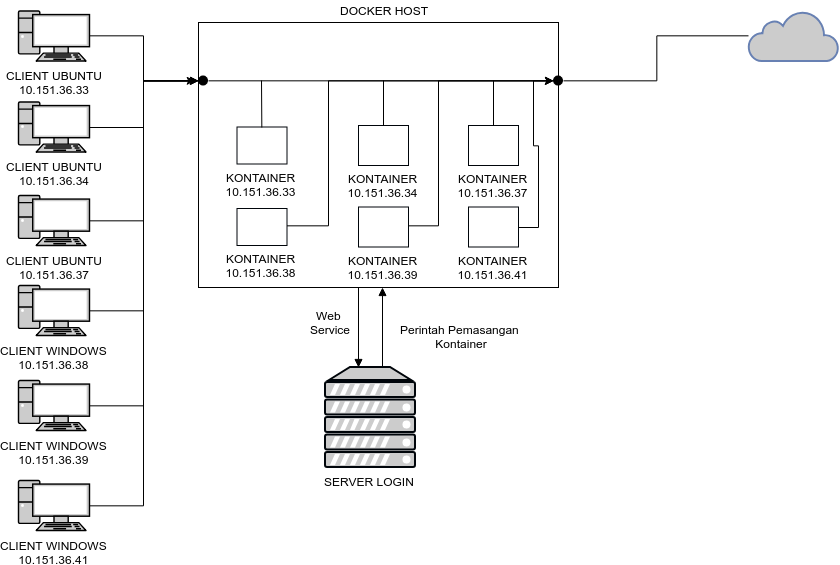
\includegraphics[width=\linewidth]{images/bab5/arsitekturbab5}
				\caption{Arsitektur dari Setiap Komponen Uji Coba}
				\label{arsitekturbab5}
			\end{figure}
			
   
\section{Skenario Uji Coba} \label{skenarioujicoba}
	Uji coba akan dilakukan untuk mengetahui keberhasilan sistem yang telah dibangun. Skenario pengujian dibedakan menjadi 2 bagian, yaitu:
    \begin{itemize}
    \item \textbf{Uji Fungsionalitas} \\
    	Pengujian ini didasarkan pada fungsionalitas yang disajikan sistem.
    \item \textbf{Uji Performa} \\
    	Pengujian ini untuk menguji ketahanan sistem terhadap sejumlah permintaan ke aplikasi secara bersamaan. Pengujian dilakukan dengan melakukan \textit{benchmark} pada sistem.
    \end{itemize}
    
\subsection{Skenario Uji Coba Fungsionalitas}
Uji coba fungsionalitas dilakukan dengan cara menjalankan sistem yang telah dibuat, dan melakukan pengujian terhadap fitur yang telah dibuat. Uji coba fungsionalitas akan berfungsi untuk memastikan sistem sudah memenuhi kebutuhan yang tertera pada Bab 3, yaitu meliputi:

\begin{enumerate}
\item Pengujian \textit{client} dapat mengakses internet.
\item Pengujian fungsionalitas menu aplikasi halaman administrator.
\end{enumerate}

\subsubsection{Uji \textit{client} dapat Mengakses Internet} \label{keempat}
Pengujian ini dilakukan untuk mengetahui apakah \textit{client} dapat mengakses internet atau tidak. Pada uji \textit{client} dapat mengakses internet akan dibagi lagi menjadi beberapa bagian, antara lain:
\begin{enumerate}
\item Pengujian \textit{client} dapat \textit{login} ke dalam sistem.
\item Pengujian \textit{client} dapat mengirimkan permintaan penyediaan kontainer \textit{docker} ke \textit{docker host}.
\item Pengujian \textit{docker host} dapat menerima permintaan penyediaan kontainer \textit{docker}.
\end{enumerate}

Pengujian menggunakan enam buah komputer penguji. Pengujian ini dapat dilakukan dengan membuka \textit{browser} dan membuka \textit{website} HTTP ataupun juga HTTPS. Daftar uji fungsionalitas \textit{client} dapat mengakses internet dijelaskan pada Tabel \ref{ujicoba4}.
\begin{longtable}{|p{0.05\textwidth}|p{0.38\textwidth}|p{0.39\textwidth}|}					\caption{Skenario Uji \textit{Client} dapat Mengakses Internet} \label{ujicoba4} \\
	\hline
	\textbf{No} & \textbf{Uji Coba} & \textbf{Hasil Harapan} \\ \hline
	\endfirsthead
	\caption[]{Skenario Uji Mengelola Aplikasi Berbasis Docker} \\
	\hline
	\textbf{No} & \textbf{Uji Coba} & \textbf{Hasil Harapan} \\ \hline
	\endhead
	\endfoot
	\endlastfoot
	
	1 & \textit{Client} membuka website HTTP maupun HTTPS dengan menggunakan \textit{browser}. & \textit{Client} dapat membuka website HTTP maupun HTTPS dengan menggunakan \textit{browser} yang ada.\\ \hline
\end{longtable}

\paragraph{Uji \textit{Client} dapat \textit{Login} ke Dalam Sistem} \label{pertama}
Pengujian ini dilakukan untuk mengetahui apakah \textit{client} sudah bisa \textit{login} ke dalam sistem saat \textit{client} akan mengakses internet. Pengujian menggunakan satu buah \textit{server} yang berperan sebagai \textit{server login} untuk \textit{client} dan menggunakan enam buah Komputer Penguji yang dijalankan dengan VirtualBox berperan sebagai \textit{client}. Pengujian dilakukan oleh \textit{client} dalam keadaan belum \textit{login} ke dalam sistem. Ketika \textit{client} mencoba membuka sebuah web, maka \textit{client} akan diarahkan ke \textit{server login} terlebih dahulu.

Alamat / IP \textit{address} dari \textit{server login} yang digunakan adalah \texttt{10.151.36.173}. Setelah \textit{client} diarahkan ke \textit{server login}, selanjutnya adalah \textit{client} harus memasukkan \textit{input username} dan \textit{password}. Daftar uji fungsionalitas \textit{client} dapat \textit{login} ke dalam sistem dijelaskan pada Tabel \ref{ujicoba1}

\begin{longtable}{|p{0.05\textwidth}|p{0.38\textwidth}|p{0.39\textwidth}|}					\caption{Skenario Uji \textit{Client} dapat \textit{Login} ke Dalam Sistem} \label{ujicoba1} \\
	\hline
	\textbf{No} & \textbf{Uji Coba} & \textbf{Hasil Harapan} \\ \hline
	\endfirsthead
	\caption[]{Skenario Uji Mengelola Aplikasi Berbasis Docker} \\
	\hline
	\textbf{No} & \textbf{Uji Coba} & \textbf{Hasil Harapan} \\ \hline
	\endhead
	\endfoot
	\endlastfoot
	
	1 & \textit{Client} membuka sebuah website ketika belum \textit{login} ke dalam sistem. & \textit{Traffic} dari \textit{client} akan diarahkan ke \textit{server login} dan \textit{client} dapat membuka halaman \textit{login} secara otomatis.\\ \hline
	2 & \textit{Client} melakukan \textit{login} ke \textit{server login}. & \textit{Client} berhasil melakukan \textit{login} dengan menggunakan \textit{username} dan \textit{password} yang sudah ditentukan.\\ \hline
\end{longtable}

\paragraph{Uji \textit{Client} dapat Mengirimkan Permintaan Penyediaan Kontainer \textit{Docker} ke \textit{Docker Host}} \label{kedua}
Pengujian ini dilakukan untuk memberikan perintah kepada \textit{docker host} untuk menyediakan kontainer \textit{docker} ke \textit{client} yang baru saja berhasil \textit{login} ke dalam sistem. Pengujian menggunakan satu buah \textit{server} yang berperan sebagai \textit{server login} yang akan mengirimkan permintaan penyediaan kontainer \textit{docker} ke \textit{docker host}.

Pengujian ini dapat dilakukan setelah \textit{client} berhasil memasukkan \textit{username} dan \textit{password} ke sistem, dan berhasil \textit{login} ke dalam sistem. Setelah itu sistem akan mengirimkan permintaan penyediaan kontainer \textit{docker} ke \textit{docker host}. Daftar uji fungsionalitas \textit{client} dapat mengirimkan permintaan penyediaan kontainer \textit{docker} ke \textit{docker} host dijelaskan pada Tabel \ref{ujicoba2}

\begin{longtable}{|p{0.05\textwidth}|p{0.38\textwidth}|p{0.39\textwidth}|}					\caption{Skenario Uji \textit{Client} dapat \textit{Login} Mengirimkan Permintaan Penyediaan Kontainer \textit{Docker}} \label{ujicoba2} \\
	\hline
	\textbf{No} & \textbf{Uji Coba} & \textbf{Hasil Harapan} \\ \hline
	\endfirsthead
	\caption[]{Skenario Uji Mengelola Aplikasi Berbasis Docker} \\
	\hline
	\textbf{No} & \textbf{Uji Coba} & \textbf{Hasil Harapan} \\ \hline
	\endhead
	\endfoot
	\endlastfoot
	
	1 & \textit{Client} mengirimkan permintaan penyediaan kontainer \textit{docker} kepada \textit{docker host}. & \textit{Client} berhasil mengirimkan permintaan penyediaan kontainer \textit{docker} kepada \textit{docker host}.\\ \hline
\end{longtable}

\paragraph{Uji \textit{Docker Host} dapat Menerima Permintaan Penyediaan Kontainer \textit{Docker}} \label{ketiga}
Pengujian ini dilakukan untuk menerima perintah permintaan penyediaan kontainer \textit{docker} pada \textit{docker host}. Pengujian menggunakan satu buah \textit{server} yang berperan sebagai \textit{docker host} yang akan menerima permintaan penyediaan kontainer \textit{docker}.

Alamat dari \textit{server} yang berperan sebagai \textit{docker host} adalah \texttt{10.151.36.134}. Setelah berhasil menerima permintaan penyediaan kontainer \textit{docker}, selanjutnya adalah sistem akan menuliskan \textit{username}, IP \textit{address}, dan \textit{port} dari \textit{client} yang telah mengirimkan permintaan penyediaan kontainer \textit{docker} ke basis data yang sudah tersedia.

Setelah selesai menuliskan \textit{username}, IP \textit{address}, dan \textit{port} dari \textit{client} yang telah mengirimkan permintaan penyediaan kontainer \textit{docker} ke basis data yang sudah tersedia, selanjutnya adalah membuat satu buah kontainer \textit{docker} dengan nama kontainer \texttt{[IP-Username-Port]}, dimana \texttt{IP} adalah IP \textit{address} dari \textit{client}, \texttt{Username} adalah \textit{username} ketika \textit{client} memasukkan \textit{inputan} kepada sistem saat akan \textit{login}, dan \texttt{Port} adalah sebuah \textit{port} khusus untuk \textit{client} tersebut.

Terakhir, pengujian yang dilakukan adalah membuat sebuah \textit{directory} pada \textit{docker host} yang berfungsi untuk menyimpan data \textit{log traffic} dari \textit{client}. \textit{Directory} ini akan dibuat pada \texttt{/container-data/[Tanggal]/[IP-USERNAME-PORT]}, dimana \texttt{Tanggal} akan sesuai dengan tanggal ketika \textit{client} berhasil \textit{login} ke dalam sistem, dan \texttt{[IP-USERNAME-PORT]} sesuai dengan yang sudah dituliskan pada basis data.

Daftar uji fungsionalitas \textit{docker host} dapat menerima permintaan penyediaan kontainer \textit{docker} dijelaskan pada Tabel \ref{ujicoba3}.

\begin{longtable}{|p{0.05\textwidth}|p{0.38\textwidth}|p{0.39\textwidth}|}					\caption{Skenario Uji \textit{Docker Host} dapat Menerima Permintaan Penyediaan Kontainer \textit{Docker}} \label{ujicoba3} \\
	\hline
	\textbf{No} & \textbf{Uji Coba} & \textbf{Hasil Harapan} \\ \hline
	\endfirsthead
	\caption[]{Skenario Uji Mengelola Aplikasi Berbasis Docker} \\
	\hline
	\textbf{No} & \textbf{Uji Coba} & \textbf{Hasil Harapan} \\ \hline
	\endhead
	\endfoot
	\endlastfoot
	
	1 & Sistem menerima permintaan penyediaan kontainer \textit{docker} dari \textit{client} pada \textit{docker host}. & Sistem berhasil menerima permintaan penyediaan kontainer \textit{docker} dari \textit{client} dan menuliskannya pada basis data pada \textit{docker host}.\\ \hline
	2 & Sistem membuat satu buah kontainer \textit{docker} untuk \textit{client} pada \textit{docker host}. & Sistem berhasil membuat satu buah kontainer \textit{docker} dengan nama sesuai yang ditulis pada basis data untuk \textit{client} yang berisi Mitmproxy pada \textit{docker host}.\\ \hline
	3 & Sistem membuat sebuah \textit{directory} pada \textit{docker host} sesuai dengan tanggal dan informasi dari \textit{client}. & Sistem berhasil membuat sebuah \textit{directory} pada \textit{docker host} sesuai dengan tanggal dan informasi dari \textit{client} yang sudah dituliskan pada basis data.\\ \hline
\end{longtable}

\subsubsection{Uji Fungsionalitas Menu Aplikasi Halaman \textit{Administrator}} \label{kelima}
Aplikasi halaman \textit{administrator} digunakan untuk membaca \textit{log traffic} dari \textit{client} yang sedang mengakses internet dan juga untuk melihat rekap \textit{client} yang telah menggunakan internet pada hari-hari sebelumnya. Aplikasi halaman \textit{administraotr} terdiri dari dua bagian utama, yaitu halaman \textit{user list}, dan \textit{history}. Rancangan pengujian dan hasil yang diharapkan ditunjukkan dengan Tabel \ref{ujicoba5}.

\begin{longtable}{|p{0.05\textwidth}|p{0.20\textwidth}|p{0.30\textwidth}|p{0.27\textwidth}|}
	\caption{Skenario Uji Fungsionalitas Aplikasi Halaman \textit{Administrator}} \label{ujicoba5} \\
	\hline
	\textbf{No} & \textbf{Menu} & \textbf{Uji Coba} & \textbf{Hasil Harapan} \\ \hline
	\endfirsthead
	\caption[]{Skenario Uji Fungsionalitas Aplikasi Dasbor}  \\
	\hline
	\textbf{No} & \textbf{Menu} & \textbf{Uji Coba} & \textbf{Hasil Harapan} \\ \hline
	\endhead
	\endfoot
	\endlastfoot
	1 & User List & Menampilkan halaman \textit{user list} pada web. & Halaman \textit{user list} dapat tampil pada web. \\ \cline{3-4}
	&& Melihat secara \textit{live} atau langsung \textit{log traffic} dari \textit{client}. & \textit{User} yang mempunyai akses membuka halaman \textit{administrator} dapat melihat secara \textit{live} atau langsung \textit{log traffic} dari \textit{client}. \\ \cline{3-4}
	&& Melihat \textit{log traffic} terakhir dari \textit{client}. & \textit{User} yang mempunyai akses membuka halaman \textit{administrator} dapat melihat \textit{log traffic} terakhir dari \textit{client}. \\ \hline
	2 & History & Melihat \textit{log traffic} dari \textit{client} pada hari-hari sebelumnya.  & \textit{User} yang mempunyai akses membuka halaman \textit{administrator} dapat melihat \textit{log traffic} dari \textit{client} pada hari-hari sebelumnya. \\ \hline
\end{longtable}

\subsection{Skenario Uji Coba Performa}
Uji performa dilakukan dengan menggunakan enam buah desktop yang berperan sebagai \textit{client} untuk melakukan akses ke internet secara bersama-sama. \textit{Client} akan mencoba mengakses internet dengan membuka website HTTP maupun HTTPS.

Percobaan dilakukan dengan dua skenario, yaitu mengakses website HTTP dan mengakses website HTTPS

\subsubsection{Uji Performa Penggunaan \textit{Memory}}
Pengujian dilakukan dengan menghitung penggunaan \textit{memory} yang terjadi pada \textit{docker host}. Penggunaan \textit{memory} di sini adalah penggunaan dari kontainer aplikasi yang sedang berjalan. Perhitungan dilakukan dengan mengambil nilai rata-rata penggunaan \textit{memory} dari masing-masing kontainer selama proses pengujian dilakukan.

\subsubsection{Uji Performa Kecepatan Menangani \textit{Request}}
Pengujian dilakukan dengan mengukur jumlah waktu yang diperlukan untuk menyelesaikan \textit{request} yang dilakukan oleh komputer penguji. Waktu yang diukur adalah saat \textit{client} berhasil melakukan \textit{login} ke dalam sistem sampai dengan \textit{client} selesai dibuatkan sebuah kontainer \textit{docker}.

Pengujian performa kecepatan menangani \textit{request} juga dilakukan dengan membandingkan performa kecepatan dari \textit{client} ketika \textit{client} melakukan \textit{download} maupun \textit{upload} sebuah file dengan menggunakan \textit{server} internet \textit{access management} secara konvensional dengan menggunakan \textit{server} internet \textit{access management} berbasis kontainer.

\subsubsection{Uji Performa Keberhasilan \textit{Request}}
Pengujian dilakukan dengan menghitung jumlah \textit{request} atau jumlah permintaan penyediaan kontainer \textit{docker} yang gagal dilakukan selama skenario dijalankan. Dari semua jumlah \textit{request} yang dikirimkan selama pengujian, akan didapatkan persen \textit{request} yang gagal dilakukan.
    
\section{Hasil Uji Coba dan Evaluasi}
Berikut dijelaskan hasil uji coba dan evaluasi berdasarkan skenario yang telah dijelaskan pada subbab \ref{skenarioujicoba}.
    
\subsection{Uji Fungsionalitas}
Berikut dijelaskan hasil pengujian fungsionalitas pada sistem yang dibangun.

\subsubsection{Uji \textit{Client} dapat Mengakses Internet}
Pengujian dilakukan sesuai dengan skenario yang dijelaskan pada subbab \ref{keempat} dan pada Tabel \ref{ujicoba4}. Pada hasil uji \textit{client} dapat mengakses internet akan dibagi lagi menjadi beberapa bagian, antara lain
\begin{enumerate}
\item Pengujian \textit{client} dapat \textit{login} ke dalam sistem.
\item Pengujian \textit{client} dapat mengirimkan permintaan penyediaan kontainer \textit{docker} ke \textit{docker host}.
\item Pengujian \textit{docker host} dapat menerima permintaan penyediaan kontainer \textit{docker}.
\end{enumerate}

Setelah melalui hasil uji yang telah disebutkan diatas, hasil pengujian \textit{client} dapat mengakses internet seperti tertera pada Tabel \ref{hasilujicoba5}

\begin{longtable}{|p{0.05\textwidth}|p{0.55\textwidth}|p{0.22\textwidth}|}					\caption{Hasil Uji Coba \textit{Client} dapat Mengakses Internet} \label{hasilujicoba5} \\
	\hline
	\textbf{No} & \textbf{Uji Coba} & \textbf{Hasil} \\ \hline
	\endfirsthead
	\caption[]{Hasil Uji Coba Mengelola Aplikasi Berbasis Docker} \\
	\hline
	\textbf{No} & \textbf{Uji Coba} & \textbf{Hasil} \\ \hline
	\endhead
	\endfoot
	\endlastfoot
	
	1 & \textit{Client} membuka sebuah website HTTP maupun HTTPS dengan menggunakan \textit{browser}. & OK. \\ \hline
\end{longtable}
Sesuai dengan skenario uji coba  yang diberikan pada Tabel \ref{ujicoba4}, hasil uji coba menunjukkan semua skenario berhasil ditangani.


\paragraph{Uji \textit{Client} dapat \textit{Login} ke Dalam Sistem}
Pengujian dilakukan sesuai dengan skenario yang dijelaskan pada subbab \ref{pertama} dan pada Tabel \ref{ujicoba1}. Hasil pengujian seperti tertera pada Tabel \ref{hasilujicoba1}.
        
\begin{longtable}{|p{0.05\textwidth}|p{0.55\textwidth}|p{0.22\textwidth}|}					\caption{Hasil Uji Coba \textit{Client} dapat \textit{Login} ke Dalam Sistem} \label{hasilujicoba1} \\
	\hline
	\textbf{No} & \textbf{Uji Coba} & \textbf{Hasil} \\ \hline
	\endfirsthead
	\caption[]{Hasil Uji Coba Mengelola Aplikasi Berbasis Docker} \\
	\hline
	\textbf{No} & \textbf{Uji Coba} & \textbf{Hasil} \\ \hline
	\endhead
	\endfoot
	\endlastfoot
	
    1 & \textit{Client} membuka sebuah website ketika belum \textit{login} ke dalam sistem. & OK. \\ \hline
    2 & \textit{Client} melakukan \textit{login} ke \textit{server login}. & OK. \\ \hline
\end{longtable}
Sesuai dengan skenario uji coba  yang diberikan pada Tabel \ref{ujicoba1}, hasil uji coba menunjukkan semua skenario berhasil ditangani.

\paragraph{Uji \textit{Client} dapat Mengirimkan Permintaan Penyediaan Kontainer \textit{Docker} ke \textit{Docker Host}}
Pengujian dilakukan sesuai dengan skenario yang dijelaskan pada subbab \ref{kedua} dan pada Tabel \ref{ujicoba2}. Hasil pengujian seperti tertera pada Tabel \ref{hasilujicoba2}.

\begin{longtable}{|p{0.05\textwidth}|p{0.55\textwidth}|p{0.22\textwidth}|}					\caption{Hasil Uji Coba \textit{Client} dapat Mengirimkan Permintaan Penyediaan Kontainer \textit{Docker} ke \textit{Docker Host}} \label{hasilujicoba2} \\
	\hline
	\textbf{No} & \textbf{Uji Coba} & \textbf{Hasil} \\ \hline
	\endfirsthead
	\caption[]{Hasil Uji Coba Mengelola Aplikasi Berbasis Docker} \\
	\hline
	\textbf{No} & \textbf{Uji Coba} & \textbf{Hasil} \\ \hline
	\endhead
	\endfoot
	\endlastfoot
	
	1 & \textit{Client} mengirimkan permintaan penyediaan kontainer \textit{docker} kepada \textit{docker host}. & OK. \\ \hline
\end{longtable}
Sesuai dengan skenario uji coba  yang diberikan pada Tabel \ref{ujicoba2}, hasil uji coba menunjukkan semua skenario berhasil ditangani.

\paragraph{Uji \textit{Docker Host} dapat Menerima Permintaan Penyediaan Kontainer \textit{Docker}}
Pengujian dilakukan sesuai dengan skenario yang dijelaskan pada subbab \ref{ketiga} dan pada Tabel \ref{ujicoba3}. Hasil pengujian seperti tertera pada Tabel \ref{hasilujicoba3}.

\begin{longtable}{|p{0.05\textwidth}|p{0.55\textwidth}|p{0.22\textwidth}|}					\caption{Hasil Uji Coba \textit{Docker Host} dapat Menerima Permintaan Penyediaan Kontainer \textit{Docker}} \label{hasilujicoba3} \\
	\hline
	\textbf{No} & \textbf{Uji Coba} & \textbf{Hasil} \\ \hline
	\endfirsthead
	\caption[]{Hasil Uji Coba Mengelola Aplikasi Berbasis Docker} \\
	\hline
	\textbf{No} & \textbf{Uji Coba} & \textbf{Hasil} \\ \hline
	\endhead
	\endfoot
	\endlastfoot
	
	1 & Sistem menerima permintaan penyediaan kontainer \textit{docker} dari \textit{client} pada \textit{docker host}. & OK. \\ \hline
	2 & Sistem membuat satu buah kontainer \textit{docker} untuk \textit{client} pada \textit{docker host}. & OK. \\ \hline
	3 & Sistem membuat sebuah \textit{directory} pada \textit{docker host} sesuai dengan tanggal dan informasi dari \textit{client}. & OK. \\ \hline
\end{longtable}
Sesuai dengan skenario uji coba  yang diberikan pada Tabel \ref{ujicoba3}, hasil uji coba menunjukkan semua skenario berhasil ditangani.
        
\subsubsection{Uji Fungsionalitas Menu Aplikasi Halaman \textit{Administrator}}
Pengujian dilakukan sesuai dengan skenario yang dijelaskan pada subbab \ref{kelima} dan pada Tabel \ref{ujicoba5}. Hasil pengujian seperti tertera pada Tabel \ref{hasilujicoba6}

\begin{longtable}{|p{0.05\textwidth}|p{0.20\textwidth}|p{0.30\textwidth}|p{0.27\textwidth}|}
	\caption{Hasil Uji Fungsionalitas Aplikasi Halaman \textit{Administrator}} \label{hasilujicoba6} \\
	\hline
	\textbf{No} & \textbf{Menu} & \textbf{Uji Coba} & \textbf{Hasil Harapan} \\ \hline
	\endfirsthead
	\caption[]{Hasil Uji Fungsionalitas Aplikasi Halaman \textit{Administrator}}  \\
	\hline
	\textbf{No} & \textbf{Menu} & \textbf{Uji Coba} & \textbf{Hasil} \\ \hline
	\endhead
	\endfoot
	\endlastfoot
	1 & User List & Menampilkan halaman \textit{user list} pada web. & OK. \\ \cline{3-4}
	&& Melihat secara \textit{live} atau langsung \textit{log traffic} dari \textit{client}. & OK. \\ \cline{3-4}
	&& Melihat \textit{log traffic} terakhir dari \textit{client}. & OK. \\ \hline
	2 & History & Melihat \textit{log traffic} dari \textit{client} pada hari-hari sebelumnya.  & OK. \\ \hline
\end{longtable}

Sesuai dengan skenario uji coba yang diberikan pada Tabel \ref{ujicoba5}, hasil uji coba menunjukkan semua skenario berhasil ditangani.

\subsection{Hasil Uji Performa}
Seperti yang sudah dijelaskan pada subbab \ref{skenarioujicoba} pengujian performa dilakukan dengan menggunakan enam buah \textit{desktop} yang berperan sebagai \textit{client} untuk melakukan akses ke internet secara bergantian. \textit{Client} akan mencoba mengakses internet dengan membuka \textit{website} HTTP maupun HTTPS.

\subsubsection{Penggunaan \textit{Memory}}
Pengujian dilakukan dengan menghitung penggunaan \textit{memory} yang terjadi pada \textit{docker host}. Penggunaan \textit{memory} di sini adalah penggunaan dari kontainer aplikasi yang sedang berjalan. Perhitungan dilakukan dengan mengambil nilai rata-rata penggunaan \textit{memory} dari masing-masing kontainer selama proses pengujian dilakukan.

\subsubsection{Kecepatan Menangani \textit{Request}}
Pengujian dilakukan dengan mengukur jumlah waktu yang diperlukan untuk menyelesaikan \textit{request} yang dilakukan oleh komputer penguji. Waktu yang diukur adalah saat \textit{client} berhasil melakukan \textit{login} ke dalam sistem sampai dengan \textit{client} selesai dibuatkan sebuah kontainer \textit{docker}.

Pengujian juga dilakukan dengan mengukur kecepatan unduh dan juga upload dari \textit{client}. Waktu yang diukur adalah saat \textit{client} mencoba mengunduh beberapa \textit{file} dari salah satu \textit{server}.

\subsubsection{Keberhasilan \textit{Request}}
Pengujian dilakukan dengan menghitung jumlah \textit{request} atau jumlah permintaan penyediaan kontainer \textit{docker} yang gagal dilakukan selama skenario dijalankan. Dari semua jumlah \textit{request} yang dikirimkan selama pengujian, akan didapatkan persen \textit{request} yang gagal dilakukan.

\section{Hasil Uji Coba dan Evaluasi}
Berikut dijelaskan hasil uji coba dan evaluasi berdasarkan skenario yang telah dijelaskan pada subbab \ref{skenarioujicoba}.

\subsection{Hasil Uji Performa}
Seperti yang sudah dijelaskan pada subbab \ref{skenarioujicoba} pengujian performa dilakukan dengan menggunakan enam buah desktop yang berperan sebagai \textit{client} untuk melakukan akses ke internet secara bergantian. \textit{Clint} akan mencoba mengakses internet dengan membuka website HTTP maupun HTTPS.

\subsubsection{Kecepatan Menangani \textit{Request}}
Dari hasil uji coba kecepatan menangani \textit{request}, yaitu kecepatan unduh dan \textit{upload} dari \textit{client}. Uji coba dilakukan dengan melakukan cek kecepatan pada website \texttt{http://www.speedtest.net/id}. Uji coba dilakukan dengan menggunakan satu komputer penguji sampai dengan enam komputer penguji secara bersamaan. Hasil dari uji coba menangani \textit{request} dapat dilihat pada Tabel \ref{kecepatanrequest2}.

\begin{longtable}{|p{0.2\textwidth}|p{0.25\textwidth}|p{0.25\textwidth}|p{0.2\textwidth}|}
	\caption{Kecepatan Menangai \textit{Request} Unduh dan \textit{Upload} Menggunakan Internet \textit{Access Management} Berbasis Kontainer} \label{kecepatanrequest2} \\
	\hline
	\textbf{Jumlah Client} & \textbf{Kecepatan unduh} & \textbf{Kecepatan \textit{Upload}} \\ \hline
	\endfirsthead
	\caption[]{Kecepatan Menangai \textit{Request} Unduh} \\
	\hline
	\endhead
	\endfoot
	\endlastfoot
	
	1 & $\pm$ 13,04 Mb & $\pm$ 13,62 Mb \\ \hline
	2 & $\pm$ 10,16 Mb & $\pm$ 9,27 Mb \\ \hline
	3 & $\pm$ 4,73 Mb & $\pm$ 4,47 Mb \\ \hline
	4 & $\pm$ 4,45 MB & $\pm$ 5,61 Mb \\ \hline
	5 & $\pm$ 3,93 MB & $\pm$ 4,55 Mb \\ \hline
	6 & $\pm$ 2,82 MB & $\pm$ 2,73 Mb \\ \hline
	
\end{longtable}

Hasil uji coba kecepatan menangani \textit{request} dengan menggunakan Internet \textit{Access Management} berbasis kontainer ditunjukkan dalam grafik pada Gambar \ref{grafikkecepatan1}.

\begin{figure}[H]
	\centering
	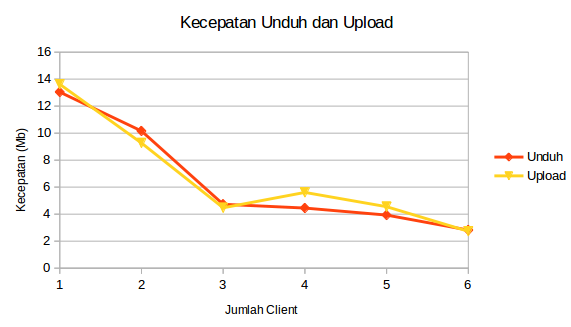
\includegraphics[width=\linewidth]{images/bab5/kecepatan1}
	\caption{Grafik Kecepatan Menangani \textit{Request}}
	\label{grafikkecepatan1}
\end{figure}

Lalu untuk uji coba dilakukan dengan enam komputer penguji dan dengan menggunakan Internet \textit{Access Management} Konvensional dapat dilihat pada Tabel \ref{kecepatanrequest3}

\begin{longtable}{|p{0.2\textwidth}|p{0.25\textwidth}|p{0.25\textwidth}|p{0.2\textwidth}|}
	\caption{Kecepatan Menangai \textit{Request} Unduh dan \textit{Upload} Menggunakan Internet \textit{Access Management} Konvensional} \label{kecepatanrequest3} \\
	\hline
	\textbf{Jumlah Client} & \textbf{Kecepatan unduh} & \textbf{Kecepatan \textit{Upload}} \\ \hline
	\endfirsthead
	\caption[]{Kecepatan Menangai \textit{Request} Unduh} \\
	\hline
	\endhead
	\endfoot
	\endlastfoot
	
	1 & $\pm$ 91,58 Mb & $\pm$ 91,27 Mb \\ \hline
	2 & $\pm$ 47,97 Mb & $\pm$ 51,49 Mb \\ \hline
	3 & $\pm$ 36,11 Mb & $\pm$ 35,28 Mb \\ \hline
	4 & $\pm$ 23,09 MB & $\pm$ 29,88 Mb \\ \hline
	5 & $\pm$ 22,50 MB & $\pm$ 26,20 Mb \\ \hline
	6 & $\pm$ 19,70 MB & $\pm$ 21,12 Mb \\ \hline
	
\end{longtable}

Hasil uji coba kecepatan menangani \textit{request} dengan menggunakan Internet \textit{Access Management} konvensional ditunjukkan dalam grafik pada Gambar \ref{grafikkecepatan2}.

\begin{figure}[H]
	\centering
	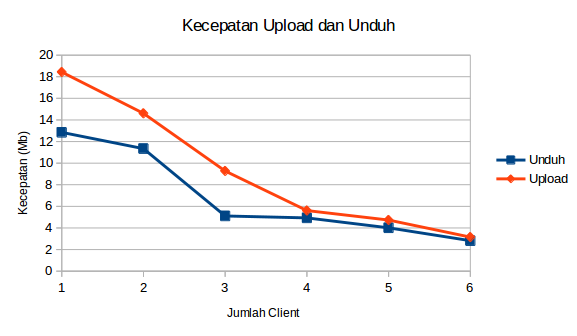
\includegraphics[width=\linewidth]{images/bab5/kecepatan2}
	\caption{Grafik Kecepatan Menangani \textit{Request}}
	\label{grafikkecepatan2}
\end{figure}

Dari Tabel \ref{kecepatanrequest2} dan Tabel \ref{kecepatanrequest3} dapat dilihat bahwa semakin banyak jumlah \textit{client}, maka semakin berkurang kecepatan unduh maupun \textit{upload} dari masing-masing \textit{client}. Hal tersebut dikarenakan \textit{bandwith} dari \textit{server} yang digunakan sebagai \textit{docker host} juga terbatas. Jika semakin besar bandwith yang dapat diterima oleh \textit{server} yang akan digunakan sebagai \textit{docker host}, maka semakin cepat pula kecepatan unduh maupun \textit{upload} dari masing-masing \textit{client}. 

\subsubsection{Penggunaan \textit{Memory}}
Dari hasil uji coba penggunaan \textit{memory}, semakin banyak \textit{request} yang diterima, semakin banyak \textit{memory} ynag diperlukan. Perhitungan penggunaan \textit{memory} adalah jumlah penggunaan dari masing-masing kontainer \textit{docker} dari \textit{client}. Dari hasil uji coba ini, dapat dilihat pada Tabel \ref{penggunaanmemory1}.

\begin{longtable}{|p{0.2\textwidth}|p{0.3\textwidth}|}
	\caption{\textit{Penggunaan \textit{Memory}}} \label{penggunaanmemory1} \\
	\hline
	\textbf{Jumlah \textit{Client}} & \textbf{Jumlah \textit{Memory} yang Digunakan} \\ \hline
	\endfirsthead

	\endhead
	\endfoot
	\endlastfoot
	
	1 & 145 MB \\ \hline
	2 & 213 MB \\ \hline
	3 & 254 MB \\ \hline
	4 & 421 MB \\ \hline
	5 & 571 MB \\ \hline
	6 & 786 MB \\ \hline
\end{longtable}
Dari Tabel \ref{penggunaanmemory1} dapat dilihat bahwa semakin banyak jumlah \textit{client} yang menggunakan Internet \textit{Access Management} berbasis kontainer, maka semakin meningkat pula penggunaan \textit{memory} dari \textit{server} yang digunakan sebagai \textit{docker host}. Rata-rata penggunaan \textit{memory} dari tiap kontainer \textit{docker} adalah sebesar $\pm$ 131 MB. Semakin besar jumlah \textit{memory} yang ada di \textit{docker host}, maka semakin banyak pula jumlah \textit{client} yang dapat ditampung.

Penggunaan \textit{memory} dari tiap kontainer juga dapat dibatasi oleh sistem jika \textit{docker host} yang digunakan hanya mempunyai \textit{memory} yang tidak terlalu besar. Hasil uji coba penggunaan \textit{memroy} ditunjukkan dalam grafik pada Gambar \ref{ram1}.

\begin{figure}[H]
	\centering
	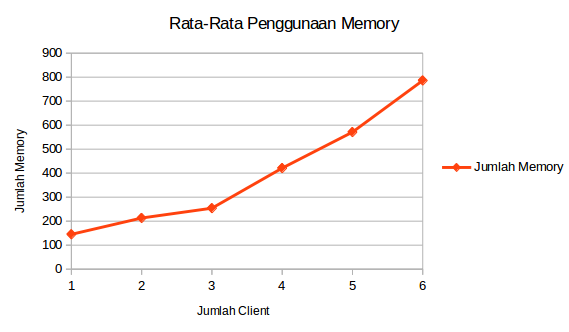
\includegraphics[width=\linewidth]{images/bab5/ram1}
	\caption{Grafik Penggunaan \textit{Memory}}
	\label{ram1}
\end{figure}

\subsubsection{Keberhasilan \textit{Request}}
Pada uji coba ini, dilakukan perhitungan seberapa besar jumlah \textit{request} yang berhasil dilakukan. Untuk jumlah \textit{client}, dapat dilihat pada Tabel \ref{keberhasilanrequest1}.

\begin{longtable}{|p{0.3\textwidth}|p{0.3\textwidth}|}
	\caption{\textit{Success Ratio Request}} \label{keberhasilanrequest1} \\
	\hline
	\textbf{\textit{Client}} & \textbf{Persen Sukses} \\ \hline
	\endfirsthead
	\caption[]{\textit{Success Ratio Request}} \\
	\hline
	\textbf{\textit{Client}} & \textbf{Persen Sukses} \\ \hline
	\endhead
	\endfoot
	\endlastfoot
	
	\textit{Client} 1 & 100\% \\ \hline
	\textit{Client} 2 & 100\% \\ \hline
	\textit{Client} 3 & 100\% \\ \hline
	\textit{Client} 4 & 100\% \\ \hline
	\textit{Client} 5 & 100\% \\ \hline
	\textit{Client} 6 & 100\% \\ \hline
\end{longtable}
Dari Tabel \ref{keberhasilanrequest1} dapat dilihat bahwa semua \textit{request} dari \textit{client} sukses dijalankan dan tidak ada \textit{error} sama sekali. Hasil uji coba tersebut berdasarkan keberhasilan \textit{client} untuk mengakses internet, mulai dari \textit{client} login ke dalam sistem sampai dengan sistem menyediakan sebuah kontainer \textit{docker} untuk \textit{client tersebut} dan berdasarkan keberhasilan \textit{client} untuk mengakses website HTTP maupun HTTPS.